\documentclass[12pt]{article}

\usepackage{amssymb,amsmath,dsfont,amsfonts,eurosym,geometry,ulem,graphicx,caption,subcaption,color,setspace,sectsty,comment,footmisc,natbib,pdflscape,subfigure,array,hyperref, enumitem}
\usepackage{booktabs}
\usepackage[para,online,flushleft]{threeparttable}
\usepackage{tikz}

\usepackage{listings}
\usepackage{xcolor}

\definecolor{codegreen}{rgb}{0,0.6,0}
\definecolor{codegray}{rgb}{0.5,0.5,0.5}
\definecolor{codepurple}{rgb}{0.58,0,0.82}
\definecolor{backcolour}{rgb}{0.95,0.95,0.92}
\definecolor{answerblue}{rgb}{0.0, 0.0, 0.70}

\lstset{
    backgroundcolor=\color{backcolour},   
    commentstyle=\color{codegreen},
    keywordstyle=\color{magenta},
    numberstyle=\tiny\color{codegray},
    stringstyle=\color{codepurple},
    basicstyle=\ttfamily\footnotesize,
    breakatwhitespace=false,         
    breaklines=true,                 
    captionpos=b,                    
    keepspaces=true,                 
    numbers=left,                    
    numbersep=5pt,                  
    showspaces=false,                
    showstringspaces=false,
    showtabs=false,                  
    tabsize=2
}

\begin{document}

\title{Writing Notes}
 \date{}
\maketitle
\section{YZ: 3/11/2026}

\subsection{Estimation Results}
\begin{enumerate}
    \item \textbf{Magnitude of estimated marginal costs.} 
    What is the average marginal cost of c-Si technology at the start of the sample period and at the end of the sample period? What is the average marginal cost of thin-film technology at the start of the sample period and at the end of the sample period? Could we plot a graph of the MC over the sample period, using two dotted lines to represent the two technologies?
    
    {\color{answerblue}
    The estimated base MC function (for a non-SOE, non-Zhejiang, domestic-selling firm, omitting the convex cost term $\gamma_{\text{scale}} \cdot q$) is:
    \begin{align*}
    MC^{\text{base}}_{\text{c-Si}} &= \underset{(0.499)}{2.224} \underset{(0.000)}{- 5.001} \cdot \ln(e^{GW}+1) + \underset{(0.039)}{0.144} \cdot \ln(P^{\text{poly}}) + \underset{(0.050)}{0.338} \cdot \mathbf{1}[06\text{--}08] \underset{(0.032)}{- 0.712} \cdot (t-2006) \\
    MC^{\text{base}}_{\text{thin}} &= \underset{(0.336)}{3.461} \underset{(0.446)}{- 0.110} \cdot \ln(e^{GW}+1) \underset{(0.032)}{- 0.712} \cdot (t-2006)
    \end{align*}
    where standard errors are shown in parentheses below the coefficients, $e^{GW}$ is cumulative production in GW, and $P^{\text{poly}}$ is the polysilicon spot price in \$/kg. Additionally, $\hat{\gamma}_{\text{scale}} = 3.001$ adds $3.001 \cdot q$ to MC (where $q$ is in GW), so effective MC at the firm's equilibrium output level is substantially higher than $MC^{\text{base}}$.

    \medskip
    \textit{Illustrative values} for a representative non-SOE, domestic c-Si firm with near-zero experience at the start of the sample:
    \begin{itemize}[leftmargin=2em]
        \item \textbf{Start of sample (2007):} With polysilicon at $\sim$\$200/kg:
        $MC^{\text{base}} \approx 2.224 + 0 + 0.144 \times \ln(200) + 0.338 - 0.712 \approx 2.61$ \$/W.
        \item \textbf{End of sample (2013):} With $\sim$0.1 GW cumulative experience and polysilicon at $\sim$\$20/kg:
        $MC^{\text{base}} \approx 2.224 - 0.477 + 0.431 + 0 - 4.984 \approx -2.81$ \$/W.
    \end{itemize}
    For \textbf{thin-film}: $MC^{\text{base}}_{2007} \approx 3.461 + 0.338 - 0.712 = 3.09$ \$/W; $MC^{\text{base}}_{2013} \approx 3.461 - 0.010 - 4.984 = -1.53$ \$/W.

    \medskip
    Base MC turns negative for experienced firms by 2013, driven by the combination of the time trend ($-0.712 \times 7 = -4.98$) and the c-Si experience effect. In the model, the convex cost term $\gamma_{\text{scale}} \cdot q = 3.001 \cdot q$ keeps equilibrium production finite (MC rises with output). This contributes to the model's production overprediction: total model production is 1,766 vs.\ 531 in data (+232\%).

    \medskip
     Yes, we can plot average $MC^{\text{base}}$ by year for each technology. For each firm--year observation, compute $MC^{\text{base}}_{jt}$ using the estimated parameters and the firm's actual experience and polysilicon price, then average across firms within each technology--year cell. Will send soon.
     
     Update: See below:

     Base MC is still negative in final years with the convex term, but it is less so. Also remember that export costs are relatively high, so negative base MC in China may reflect demand-side subsidies we don't capture. It should be noted that it is still positive for all but China if you account for exports.
     
\begin{figure}
    \centering
    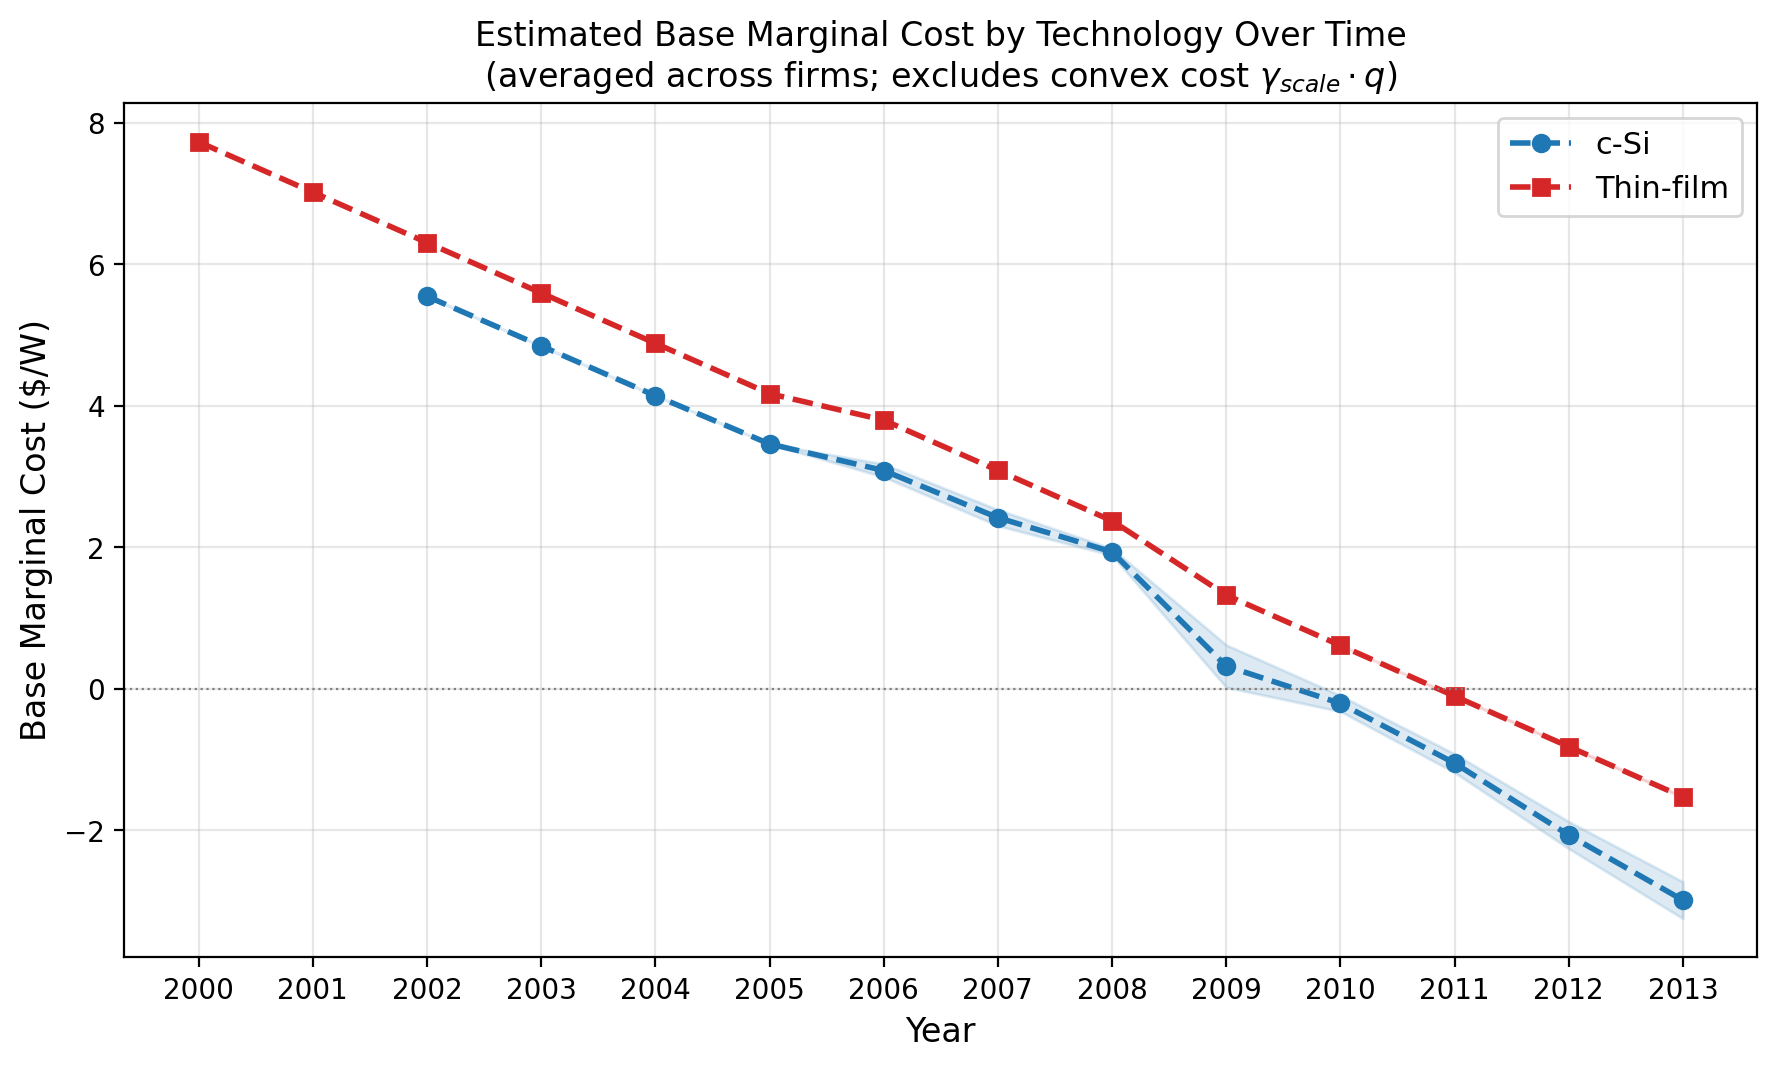
\includegraphics[width=0.5\linewidth]{Figures/mc_over_time.png}
    \caption{MC Comparison No Convex Cost}
    \label{fig:placeholder}
\end{figure}
\begin{figure}
    \centering
    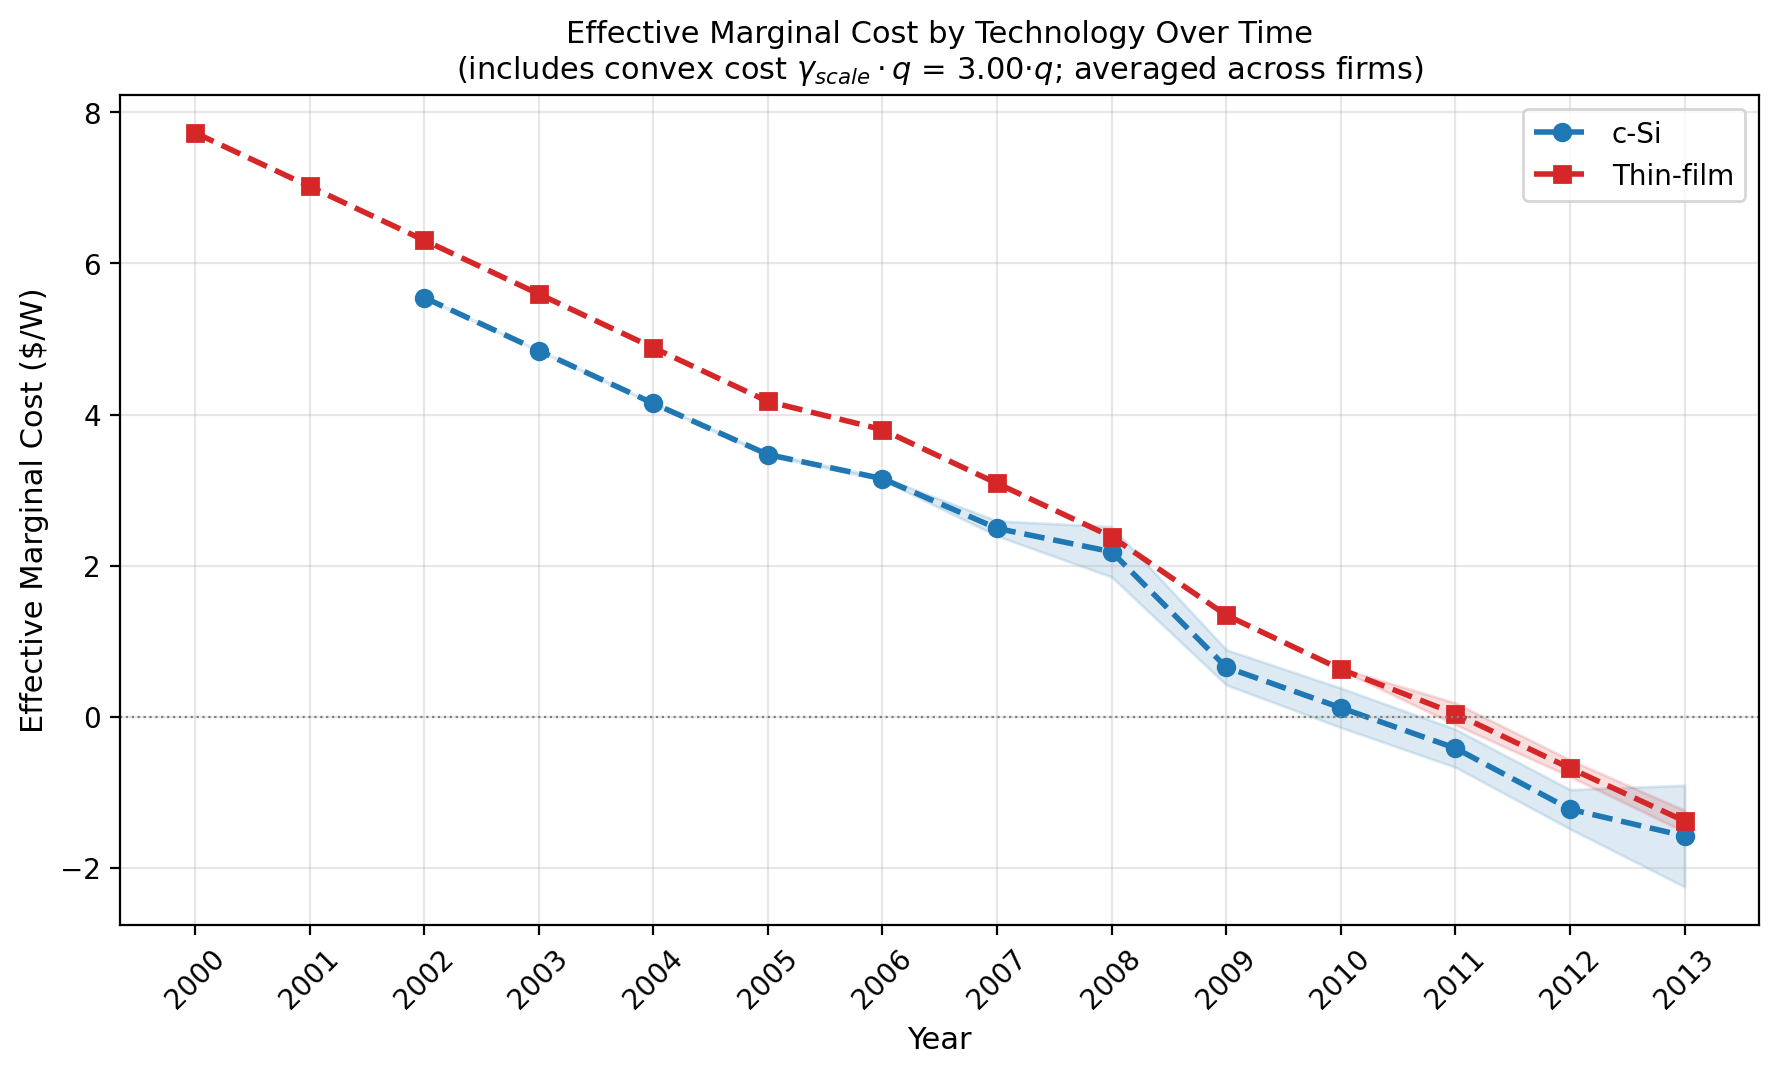
\includegraphics[width=0.5\linewidth]{Figures/mc_effective_over_time.png}
    \caption{MC Comparison with Convex Cost}
    \label{fig:placeholder}
\end{figure}
     }

     \medskip

     {\color{red} When we compute the estimated MC function, we cannot omit the convex cost term $\gamma^{scale} \cdot q$. For each year, should use the average output of all firms in that year. After bringing back this term, the MC for 2013 may no longer be negative. }

    {\color{answerblue}
See graph below. Mostly but not entirely fixed.
    }

    \item \textbf{Interpretation of experience coefficients.} 
    \begin{itemize}
        \item For c-Si manufactures, does the estimate $\gamma^{s,e} = -5.001$ indicate that doubling manufacturing experience reduces marginal cost by $ln(2)\times 5.001 = 3.466$ per MW? Given this rate, by how many dollars (\$XX) and by what percentage (XX\%) per MW have marginal costs fallen due to their cumulative experience over the sample period? 
        \item For thin film manufactures, does the estimate $\gamma^{s,e} = -1.103$ indicate that doubling manufacturing experience reduces marginal cost by $ln(2)\times 1.103 = 0.765$ per MW? Given this rate, by how many dollars (\$XX) and by what percentage (XX\%) per MW have marginal costs fallen due to their cumulative experience over the sample period?
    \end{itemize}

    {\color{answerblue}
    \begin{itemize}[leftmargin=2em]
        \item \textbf{c-Si ($\hat{\gamma}^{\text{exp}}_{\text{c-Si}} = -5.001$):} 
        The interpretation is approximately correct for firms with substantial experience ($e^{GW} \gg 1$), since $\ln(2e+1) \approx \ln(2) + \ln(e+1)$, giving $\Delta MC \approx -\ln(2) \times 5.001 = -3.466$ \$/W per doubling.

        \textit{Dollar and percentage effect over the sample:} For a firm accumulating 0.5 GW of experience over the sample: $\Delta MC = -5.001 \times [\ln(1.5) - \ln(0+1)] = -5.001 \times 0.405 = -2.03$ \$/W. Relative to an initial base MC of $\sim$2.61 \$/W, this is a 78\% reduction from learning alone. For a large firm reaching 1 GW: $\Delta MC = -5.001 \times \ln(2) = -3.47$ \$/W, exceeding 100\% of the initial base MC (which is another way of seeing why base MC turns negative).

        \item \textbf{Thin-film ($\hat{\gamma}^{\text{exp}}_{\text{thin}} = -0.110$):}
        With the current estimate, doubling experience reduces MC by only $\ln(2) \times 0.110 = 0.076$ \$/W. For a thin-film firm accumulating 0.1 GW: $\Delta MC = -0.110 \times \ln(1.1) = -0.010$ \$/W, representing $<$1\% of the initial base MC of $\sim$3.09 \$/W. This estimate is not statistically significant ($p = 0.80$), so we cannot distinguish the thin-film learning effect from zero.
        \end{itemize}
    }
    {\color{red} What is the mean level of accumulated experience over this period, taken as an average across firms of each technology?
    }

    {\color{answerblue}

    In the model's preferred log specification, $\ln(e^{GW}+1)$, the mean values are 0.118 (c-Si) and 0.050 (thin-film). These are the values that enter the marginal cost function multiplied by $\gamma_{\text{exp}}^{\tau}$. 
    
    The c-Si mean experience rises sharply in the later years (0.025 GW in 2008 to 0.683 GW in 2013), reflecting the massive production scale-up. It should be noted that a few large firms drive the mean well above the median. The median c-Si firm has only $\sim 3$ MW of cumulative experience, while the mean is 251 MW, reflecting the dominance of a handful of large producers. obviously, thin-film firms have much lower experience on average. We may not even be able to measure the effect correctly because of how low it is and because we really don't observe the large thin-film firms we do for c-Si.}

    \item \textbf{Interpretation of time trend coefficients.} Does the estimate $\gamma^{trend} = -7.116$ mean that, over the sample period, the marginal cost (MC) falls by 7.116 per MW each year? Also, the coefficient on the $2006–2008$ indicator is 3.378. Should this be interpreted as MC having risen by 3.378 per MW during $2006–2008$ ? Why is MC higher in that period, even after accounting for the effect of the polysilicon price? Alternatively, can we merge the time trend with the $2006–2008$ indicator? Do our estimates imply that MC decreases by 5.427 per year ($ = 7.116 - 0.5 \times 3.378 $) between 2006 and 2008, and then declines by 7.116 per year after 2008? If we can combine these two, what do you think about using only two trend dummy variables? Specifically, $\gamma_1^{trend} \cdot 1(t-2006) \cdot 1(t<2010)$ and $\gamma_2^{trend} \cdot 1(t-2010) \cdot 1(t \geq 2010)$, where $\gamma_1^{trend}$ represents the trend before 2010 and $\gamma_2^{trend}$ represents the trend from 2010 onward.

    {\color{answerblue}

    \begin{itemize}[leftmargin=2em]
        \item \textbf{Trend interpretation:} The term $-0.716 \cdot (t - 2006)$ implies MC declines by \$0.712/W each year, \textit{cumulatively}. Over the full sample (2007--2013), the total trend reduction is $0.716 \times 7 = 5.01$ \$/W. This captures industry-wide technological progress, supply chain maturation, and scale economies beyond firm-specific learning.

        \item \textbf{2006--2008 indicator:} This is a \textbf{level shift}, not a per-year slope. During 2006--2008, MC is elevated by 0.338 \$/W. It should be interpreted as: \textit{on top of the polysilicon price effect captured by $\gamma_{\text{poly}} \cdot \ln(P^{\text{poly}})$}, there was an additional 0.338 \$/W cost increase during the polysilicon shortage. This residual could reflect contractual rigidities such as locked-in high prices, panic stockpiling, quality degradation from alternative feedstock, or other supply-disruption costs not captured by the spot price alone.

        \item \textbf{Merging trend and indicator:} The current specification does \textit{not} imply a merged annual decline of $7.116 - 0.5 \times 3.378 = 5.427$ per year during 2006--2008. The indicator is not a slope---it is a constant level shift. The net MC path from 2006 is:
        \begin{center}
        \begin{tabular}{lccc}
        \toprule
        Year & Trend $-0.712 \times (t-2006)$ & Indicator & Net \\
        \midrule
        2006 & $0$ & $+0.338$ & $+0.338$ \\
        2007 & $-0.712$ & $+0.338$ & $-0.374$ \\
        2008 & $-1.424$ & $+0.338$ & $-1.086$ \\
        2009 & $-2.136$ & $0$ & $-2.136$ \\
        2010 & $-2.848$ & $0$ & $-2.848$ \\
        2013 & $-4.984$ & $0$ & $-4.984$ \\
        \bottomrule
        \end{tabular}
        \end{center}
        Note the discontinuity at 2009: when the indicator drops out, MC abruptly falls by 0.338.

        \item \textbf{Two-trend specification:} The suggested alternative $\gamma_1 \cdot (t-2006) \cdot \mathbf{1}[t<2010] + \gamma_2 \cdot (t-2010) \cdot \mathbf{1}[t \geq 2010]$ is a reasonable and potentially better approach. I can certainly try.
    \end{itemize}
    }

    {\color{red} My bad. There are actually three (not two) years from 2006 to 2008. Given this, our estimates suggest that MC falls by about 5.99 per year ($ = 7.116 - 3.378/3 $) over 2006–2008, and then by 7.116 per year after 2008. To obtain these rough figures, I allocate the total level change of 3.378 evenly across the three years, effectively allowing for different trends before and after 2008. The key takeaway is that the rate of decline was smaller before 2008 than it was after 2008. Can you try this new specification by allowing different time trends before and after 2010?
    }
 {\color{answerblue}

  Sure. Will run the new specification soon as I can.
 
 }

    \item \textbf{Large SEs.} Most parameters have reasonable standard errors. The exceptions are the experience parameter for thin-film technology with a SE of 4.456; the exporting costs to India and US; the SD of MC shocks with a SE of 12.835 (really high), the SD of scrap value with a SE of 2.447, and the entry cost before 2010 with a SE of 14.334 (really high). The experience parameter seems interpretable. The exporting costs and the SD of the two shocks seem acceptable. But the SE for the pre-2010 entry cost is almost twice as large as its point estimate. Could this be a typo, or is there another explanation?
    
    {\color{answerblue}

    \begin{itemize}[leftmargin=2em]
        \item \textbf{$\kappa_{\text{c-Si, pre-2010}}$: Not a typo.} The SE (0.143) exceeding the point estimate (0.079) reflects \textbf{weak identification}---the estimate is not statistically different from zero ($t = 0.55$, $p = 0.58$). The entry moment fit confirms this: the model overpredicts early c-Si entry (model = 187 vs.\ data = 96, +95\%) while underpredicting late entry (model = 133 vs.\ data = 275, $-$52\%), indicating that the entry cost parameters struggle to match the observed temporal pattern. With an entry scale of $\sigma_{\text{entry}} = \min(\max(\sigma_\phi, 0.5), 3.0) = 0.5$, entry probabilities are highly sensitive to $\kappa - CV$, creating a knife-edge identification problem for small $\kappa$.


        % \item \textbf{$\kappa_{\text{Zhejiang}} = 0$ (SE = 0):} Also at a boundary, meaning the Zhejiang entry cost adjustment is not identified from the data.

    \end{itemize}
    }
     {\color{red} If our model over-predicts entry in the early stage but under-predicts it in the later stage, we can improve the fit by raising the entry cost for the early stage and lowering it for the later stage. I don’t see how this is connected to SEs.
     }
\end{enumerate}

{\color{answerblue}
IDK. Some times things aren't significant maybe? There isn't much variation in that veriable, which may explain it. I can try to look into it?
}

\newpage
\subsection{Model Fit}

The main targets we aim to match are total output and the number of active firms over time. The estimated model should reproduce the rapid rise in output and in the number of firms prior to 2011, as well as the slowdown that followed. Therefore, we only need to show the following four figures. 
\begin{enumerate}
    \item Total output of c-Si firms over years: observed in the data and predicted by the model.
    \item Total output of thin-film firms over years: observed in the data and predicted by the model.
    \item Number of active c-Si firms over years: observed in the data and predicted by the model.
    \item Number of active thin-film firms over years: observed in the data and predicted by the model.
\end{enumerate}


\end{document}